% Created by tikzDevice version 0.12.3.1 on 2021-04-14 10:42:56
% !TEX encoding = UTF-8 Unicode
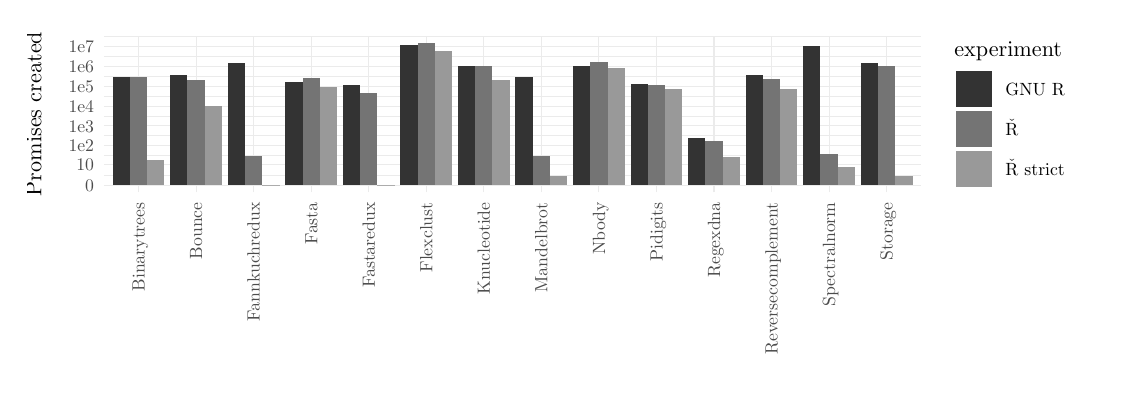
\begin{tikzpicture}[x=1pt,y=1pt]
\definecolor{fillColor}{RGB}{255,255,255}
\path[use as bounding box,fill=fillColor,fill opacity=0.00] (0,0) rectangle (390.26,130.09);
\begin{scope}
\path[clip] ( 27.60, 70.57) rectangle (322.87,127.24);
\definecolor{drawColor}{gray}{0.92}

\path[draw=drawColor,line width= 0.2pt,line join=round] ( 27.60, 76.87) --
	(322.87, 76.87);

\path[draw=drawColor,line width= 0.2pt,line join=round] ( 27.60, 84.03) --
	(322.87, 84.03);

\path[draw=drawColor,line width= 0.2pt,line join=round] ( 27.60, 91.04) --
	(322.87, 91.04);

\path[draw=drawColor,line width= 0.2pt,line join=round] ( 27.60, 98.17) --
	(322.87, 98.17);

\path[draw=drawColor,line width= 0.2pt,line join=round] ( 27.60,105.31) --
	(322.87,105.31);

\path[draw=drawColor,line width= 0.2pt,line join=round] ( 27.60,112.46) --
	(322.87,112.46);

\path[draw=drawColor,line width= 0.2pt,line join=round] ( 27.60,119.61) --
	(322.87,119.61);

\path[draw=drawColor,line width= 0.2pt,line join=round] ( 27.60,126.91) --
	(322.87,126.91);

\path[draw=drawColor,line width= 0.4pt,line join=round] ( 27.60, 73.15) --
	(322.87, 73.15);

\path[draw=drawColor,line width= 0.4pt,line join=round] ( 27.60, 80.59) --
	(322.87, 80.59);

\path[draw=drawColor,line width= 0.4pt,line join=round] ( 27.60, 87.48) --
	(322.87, 87.48);

\path[draw=drawColor,line width= 0.4pt,line join=round] ( 27.60, 94.60) --
	(322.87, 94.60);

\path[draw=drawColor,line width= 0.4pt,line join=round] ( 27.60,101.74) --
	(322.87,101.74);

\path[draw=drawColor,line width= 0.4pt,line join=round] ( 27.60,108.89) --
	(322.87,108.89);

\path[draw=drawColor,line width= 0.4pt,line join=round] ( 27.60,116.04) --
	(322.87,116.04);

\path[draw=drawColor,line width= 0.4pt,line join=round] ( 27.60,123.18) --
	(322.87,123.18);

\path[draw=drawColor,line width= 0.4pt,line join=round] ( 40.07, 70.57) --
	( 40.07,127.24);

\path[draw=drawColor,line width= 0.4pt,line join=round] ( 60.87, 70.57) --
	( 60.87,127.24);

\path[draw=drawColor,line width= 0.4pt,line join=round] ( 81.66, 70.57) --
	( 81.66,127.24);

\path[draw=drawColor,line width= 0.4pt,line join=round] (102.45, 70.57) --
	(102.45,127.24);

\path[draw=drawColor,line width= 0.4pt,line join=round] (123.25, 70.57) --
	(123.25,127.24);

\path[draw=drawColor,line width= 0.4pt,line join=round] (144.04, 70.57) --
	(144.04,127.24);

\path[draw=drawColor,line width= 0.4pt,line join=round] (164.84, 70.57) --
	(164.84,127.24);

\path[draw=drawColor,line width= 0.4pt,line join=round] (185.63, 70.57) --
	(185.63,127.24);

\path[draw=drawColor,line width= 0.4pt,line join=round] (206.42, 70.57) --
	(206.42,127.24);

\path[draw=drawColor,line width= 0.4pt,line join=round] (227.22, 70.57) --
	(227.22,127.24);

\path[draw=drawColor,line width= 0.4pt,line join=round] (248.01, 70.57) --
	(248.01,127.24);

\path[draw=drawColor,line width= 0.4pt,line join=round] (268.80, 70.57) --
	(268.80,127.24);

\path[draw=drawColor,line width= 0.4pt,line join=round] (289.60, 70.57) --
	(289.60,127.24);

\path[draw=drawColor,line width= 0.4pt,line join=round] (310.39, 70.57) --
	(310.39,127.24);
\definecolor{fillColor}{gray}{0.60}

\path[fill=fillColor] ( 63.99, 73.15) rectangle ( 70.22,101.89);

\path[fill=fillColor] ( 63.99, 73.15) rectangle ( 70.22,101.89);

\path[fill=fillColor] ( 63.99, 73.15) rectangle ( 70.22,101.89);

\path[fill=fillColor] ( 63.99, 73.15) rectangle ( 70.22,101.89);

\path[fill=fillColor] ( 63.99, 73.15) rectangle ( 70.22,101.89);

\path[fill=fillColor] ( 63.99, 73.15) rectangle ( 70.22,101.89);

\path[fill=fillColor] ( 63.99, 73.15) rectangle ( 70.22,101.89);

\path[fill=fillColor] ( 63.99, 73.15) rectangle ( 70.22,101.89);

\path[fill=fillColor] ( 63.99, 73.15) rectangle ( 70.22,101.89);

\path[fill=fillColor] ( 63.99, 73.15) rectangle ( 70.22,101.89);
\definecolor{fillColor}{RGB}{116,116,116}

\path[fill=fillColor] ( 57.75, 73.15) rectangle ( 63.99,111.06);

\path[fill=fillColor] ( 57.75, 73.15) rectangle ( 63.99,111.06);

\path[fill=fillColor] ( 57.75, 73.15) rectangle ( 63.99,111.06);

\path[fill=fillColor] ( 57.75, 73.15) rectangle ( 63.99,111.06);

\path[fill=fillColor] ( 57.75, 73.15) rectangle ( 63.99,111.06);

\path[fill=fillColor] ( 57.75, 73.15) rectangle ( 63.99,111.06);

\path[fill=fillColor] ( 57.75, 73.15) rectangle ( 63.99,111.06);

\path[fill=fillColor] ( 57.75, 73.15) rectangle ( 63.99,111.06);

\path[fill=fillColor] ( 57.75, 73.15) rectangle ( 63.99,111.06);

\path[fill=fillColor] ( 57.75, 73.15) rectangle ( 63.99,111.06);
\definecolor{fillColor}{gray}{0.20}

\path[fill=fillColor] ( 51.51, 73.15) rectangle ( 57.75,112.96);

\path[fill=fillColor] ( 51.51, 73.15) rectangle ( 57.75,112.96);

\path[fill=fillColor] ( 51.51, 73.15) rectangle ( 57.75,112.96);

\path[fill=fillColor] ( 51.51, 73.15) rectangle ( 57.75,112.96);

\path[fill=fillColor] ( 51.51, 73.15) rectangle ( 57.75,112.96);

\path[fill=fillColor] ( 51.51, 73.15) rectangle ( 57.75,112.96);

\path[fill=fillColor] ( 51.51, 73.15) rectangle ( 57.75,112.96);

\path[fill=fillColor] ( 51.51, 73.15) rectangle ( 57.75,112.96);

\path[fill=fillColor] ( 51.51, 73.15) rectangle ( 57.75,112.96);

\path[fill=fillColor] ( 51.51, 73.15) rectangle ( 57.75,112.96);
\definecolor{fillColor}{gray}{0.60}

\path[fill=fillColor] (188.75, 73.15) rectangle (194.99, 76.56);

\path[fill=fillColor] (188.75, 73.15) rectangle (194.99, 76.56);

\path[fill=fillColor] (188.75, 73.15) rectangle (194.99, 76.56);

\path[fill=fillColor] (188.75, 73.15) rectangle (194.99, 76.56);

\path[fill=fillColor] (188.75, 73.15) rectangle (194.99, 76.56);

\path[fill=fillColor] (188.75, 73.15) rectangle (194.99, 76.56);

\path[fill=fillColor] (188.75, 73.15) rectangle (194.99, 76.56);

\path[fill=fillColor] (188.75, 73.15) rectangle (194.99, 76.56);

\path[fill=fillColor] (188.75, 73.15) rectangle (194.99, 76.56);

\path[fill=fillColor] (188.75, 73.15) rectangle (194.99, 76.56);
\definecolor{fillColor}{RGB}{116,116,116}

\path[fill=fillColor] (182.51, 73.15) rectangle (188.75, 83.71);

\path[fill=fillColor] (182.51, 73.15) rectangle (188.75, 83.71);

\path[fill=fillColor] (182.51, 73.15) rectangle (188.75, 83.71);

\path[fill=fillColor] (182.51, 73.15) rectangle (188.75, 83.71);

\path[fill=fillColor] (182.51, 73.15) rectangle (188.75, 83.71);

\path[fill=fillColor] (182.51, 73.15) rectangle (188.75, 83.71);

\path[fill=fillColor] (182.51, 73.15) rectangle (188.75, 83.71);

\path[fill=fillColor] (182.51, 73.15) rectangle (188.75, 83.71);

\path[fill=fillColor] (182.51, 73.15) rectangle (188.75, 83.71);

\path[fill=fillColor] (182.51, 73.15) rectangle (188.75, 83.71);
\definecolor{fillColor}{gray}{0.20}

\path[fill=fillColor] (176.27, 73.15) rectangle (182.51,112.44);

\path[fill=fillColor] (176.27, 73.15) rectangle (182.51,112.44);

\path[fill=fillColor] (176.27, 73.15) rectangle (182.51,112.44);

\path[fill=fillColor] (176.27, 73.15) rectangle (182.51,112.44);

\path[fill=fillColor] (176.27, 73.15) rectangle (182.51,112.44);

\path[fill=fillColor] (176.27, 73.15) rectangle (182.51,112.44);

\path[fill=fillColor] (176.27, 73.15) rectangle (182.51,112.44);

\path[fill=fillColor] (176.27, 73.15) rectangle (182.51,112.44);

\path[fill=fillColor] (176.27, 73.15) rectangle (182.51,112.44);

\path[fill=fillColor] (176.27, 73.15) rectangle (182.51,112.44);
\definecolor{fillColor}{gray}{0.60}

\path[fill=fillColor] (313.51, 73.15) rectangle (319.75, 76.56);

\path[fill=fillColor] (313.51, 73.15) rectangle (319.75, 76.56);

\path[fill=fillColor] (313.51, 73.15) rectangle (319.75, 76.56);

\path[fill=fillColor] (313.51, 73.15) rectangle (319.75, 76.56);

\path[fill=fillColor] (313.51, 73.15) rectangle (319.75, 76.56);

\path[fill=fillColor] (313.51, 73.15) rectangle (319.75, 76.56);

\path[fill=fillColor] (313.51, 73.15) rectangle (319.75, 76.56);

\path[fill=fillColor] (313.51, 73.15) rectangle (319.75, 76.56);

\path[fill=fillColor] (313.51, 73.15) rectangle (319.75, 76.56);

\path[fill=fillColor] (313.51, 73.15) rectangle (319.75, 76.56);
\definecolor{fillColor}{RGB}{116,116,116}

\path[fill=fillColor] (307.27, 73.15) rectangle (313.51,116.31);

\path[fill=fillColor] (307.27, 73.15) rectangle (313.51,116.31);

\path[fill=fillColor] (307.27, 73.15) rectangle (313.51,116.31);

\path[fill=fillColor] (307.27, 73.15) rectangle (313.51,116.31);

\path[fill=fillColor] (307.27, 73.15) rectangle (313.51,116.31);

\path[fill=fillColor] (307.27, 73.15) rectangle (313.51,116.31);

\path[fill=fillColor] (307.27, 73.15) rectangle (313.51,116.31);

\path[fill=fillColor] (307.27, 73.15) rectangle (313.51,116.31);

\path[fill=fillColor] (307.27, 73.15) rectangle (313.51,116.31);

\path[fill=fillColor] (307.27, 73.15) rectangle (313.51,116.31);
\definecolor{fillColor}{gray}{0.20}

\path[fill=fillColor] (301.03, 73.15) rectangle (307.27,117.30);

\path[fill=fillColor] (301.03, 73.15) rectangle (307.27,117.30);

\path[fill=fillColor] (301.03, 73.15) rectangle (307.27,117.30);

\path[fill=fillColor] (301.03, 73.15) rectangle (307.27,117.30);

\path[fill=fillColor] (301.03, 73.15) rectangle (307.27,117.30);

\path[fill=fillColor] (301.03, 73.15) rectangle (307.27,117.30);

\path[fill=fillColor] (301.03, 73.15) rectangle (307.27,117.30);

\path[fill=fillColor] (301.03, 73.15) rectangle (307.27,117.30);

\path[fill=fillColor] (301.03, 73.15) rectangle (307.27,117.30);

\path[fill=fillColor] (301.03, 73.15) rectangle (307.27,117.30);
\definecolor{fillColor}{gray}{0.60}

\path[fill=fillColor] (147.16, 73.15) rectangle (153.40,121.58);

\path[fill=fillColor] (147.16, 73.15) rectangle (153.40,121.58);

\path[fill=fillColor] (147.16, 73.15) rectangle (153.40,121.58);

\path[fill=fillColor] (147.16, 73.15) rectangle (153.40,121.58);

\path[fill=fillColor] (147.16, 73.15) rectangle (153.40,121.58);

\path[fill=fillColor] (147.16, 73.15) rectangle (153.40,121.58);

\path[fill=fillColor] (147.16, 73.15) rectangle (153.40,121.58);

\path[fill=fillColor] (147.16, 73.15) rectangle (153.40,121.58);

\path[fill=fillColor] (147.16, 73.15) rectangle (153.40,121.58);

\path[fill=fillColor] (147.16, 73.15) rectangle (153.40,121.58);
\definecolor{fillColor}{gray}{0.20}

\path[fill=fillColor] (134.68, 73.15) rectangle (140.92,123.70);

\path[fill=fillColor] (134.68, 73.15) rectangle (140.92,123.70);

\path[fill=fillColor] (134.68, 73.15) rectangle (140.92,123.70);

\path[fill=fillColor] (134.68, 73.15) rectangle (140.92,123.70);

\path[fill=fillColor] (134.68, 73.15) rectangle (140.92,123.70);

\path[fill=fillColor] (134.68, 73.15) rectangle (140.92,123.70);

\path[fill=fillColor] (134.68, 73.15) rectangle (140.92,123.70);

\path[fill=fillColor] (134.68, 73.15) rectangle (140.92,123.70);

\path[fill=fillColor] (134.68, 73.15) rectangle (140.92,123.70);

\path[fill=fillColor] (134.68, 73.15) rectangle (140.92,123.70);
\definecolor{fillColor}{RGB}{116,116,116}

\path[fill=fillColor] (140.92, 73.15) rectangle (147.16,124.66);

\path[fill=fillColor] (140.92, 73.15) rectangle (147.16,124.66);

\path[fill=fillColor] (140.92, 73.15) rectangle (147.16,124.66);

\path[fill=fillColor] (140.92, 73.15) rectangle (147.16,124.66);

\path[fill=fillColor] (140.92, 73.15) rectangle (147.16,124.66);

\path[fill=fillColor] (140.92, 73.15) rectangle (147.16,124.66);

\path[fill=fillColor] (140.92, 73.15) rectangle (147.16,124.66);

\path[fill=fillColor] (140.92, 73.15) rectangle (147.16,124.66);

\path[fill=fillColor] (140.92, 73.15) rectangle (147.16,124.66);

\path[fill=fillColor] (140.92, 73.15) rectangle (147.16,124.66);
\definecolor{fillColor}{gray}{0.60}

\path[fill=fillColor] ( 43.19, 73.15) rectangle ( 49.43, 82.45);

\path[fill=fillColor] ( 43.19, 73.15) rectangle ( 49.43, 82.45);

\path[fill=fillColor] ( 43.19, 73.15) rectangle ( 49.43, 82.45);

\path[fill=fillColor] ( 43.19, 73.15) rectangle ( 49.43, 82.45);

\path[fill=fillColor] ( 43.19, 73.15) rectangle ( 49.43, 82.45);

\path[fill=fillColor] ( 43.19, 73.15) rectangle ( 49.43, 82.45);

\path[fill=fillColor] ( 43.19, 73.15) rectangle ( 49.43, 82.45);

\path[fill=fillColor] ( 43.19, 73.15) rectangle ( 49.43, 82.45);

\path[fill=fillColor] ( 43.19, 73.15) rectangle ( 49.43, 82.45);

\path[fill=fillColor] ( 43.19, 73.15) rectangle ( 49.43, 82.45);
\definecolor{fillColor}{RGB}{116,116,116}

\path[fill=fillColor] ( 36.95, 73.15) rectangle ( 43.19,112.31);

\path[fill=fillColor] ( 36.95, 73.15) rectangle ( 43.19,112.31);

\path[fill=fillColor] ( 36.95, 73.15) rectangle ( 43.19,112.31);

\path[fill=fillColor] ( 36.95, 73.15) rectangle ( 43.19,112.31);

\path[fill=fillColor] ( 36.95, 73.15) rectangle ( 43.19,112.31);

\path[fill=fillColor] ( 36.95, 73.15) rectangle ( 43.19,112.31);

\path[fill=fillColor] ( 36.95, 73.15) rectangle ( 43.19,112.31);

\path[fill=fillColor] ( 36.95, 73.15) rectangle ( 43.19,112.31);

\path[fill=fillColor] ( 36.95, 73.15) rectangle ( 43.19,112.31);

\path[fill=fillColor] ( 36.95, 73.15) rectangle ( 43.19,112.31);
\definecolor{fillColor}{gray}{0.20}

\path[fill=fillColor] ( 30.72, 73.15) rectangle ( 36.95,112.31);

\path[fill=fillColor] ( 30.72, 73.15) rectangle ( 36.95,112.31);

\path[fill=fillColor] ( 30.72, 73.15) rectangle ( 36.95,112.31);

\path[fill=fillColor] ( 30.72, 73.15) rectangle ( 36.95,112.31);

\path[fill=fillColor] ( 30.72, 73.15) rectangle ( 36.95,112.31);

\path[fill=fillColor] ( 30.72, 73.15) rectangle ( 36.95,112.31);

\path[fill=fillColor] ( 30.72, 73.15) rectangle ( 36.95,112.31);

\path[fill=fillColor] ( 30.72, 73.15) rectangle ( 36.95,112.31);

\path[fill=fillColor] ( 30.72, 73.15) rectangle ( 36.95,112.31);

\path[fill=fillColor] ( 30.72, 73.15) rectangle ( 36.95,112.31);
\definecolor{fillColor}{gray}{0.60}

\path[fill=fillColor] ( 84.78, 73.15) rectangle ( 91.02, 73.15);

\path[fill=fillColor] ( 84.78, 73.15) rectangle ( 91.02, 73.15);

\path[fill=fillColor] ( 84.78, 73.15) rectangle ( 91.02, 73.15);

\path[fill=fillColor] ( 84.78, 73.15) rectangle ( 91.02, 73.15);

\path[fill=fillColor] ( 84.78, 73.15) rectangle ( 91.02, 73.15);

\path[fill=fillColor] ( 84.78, 73.15) rectangle ( 91.02, 73.15);

\path[fill=fillColor] ( 84.78, 73.15) rectangle ( 91.02, 73.15);

\path[fill=fillColor] ( 84.78, 73.15) rectangle ( 91.02, 73.15);

\path[fill=fillColor] ( 84.78, 73.15) rectangle ( 91.02, 73.15);

\path[fill=fillColor] ( 84.78, 73.15) rectangle ( 91.02, 73.15);
\definecolor{fillColor}{RGB}{116,116,116}

\path[fill=fillColor] ( 78.54, 73.15) rectangle ( 84.78, 83.81);

\path[fill=fillColor] ( 78.54, 73.15) rectangle ( 84.78, 83.81);

\path[fill=fillColor] ( 78.54, 73.15) rectangle ( 84.78, 83.81);

\path[fill=fillColor] ( 78.54, 73.15) rectangle ( 84.78, 83.81);

\path[fill=fillColor] ( 78.54, 73.15) rectangle ( 84.78, 83.81);

\path[fill=fillColor] ( 78.54, 73.15) rectangle ( 84.78, 83.81);

\path[fill=fillColor] ( 78.54, 73.15) rectangle ( 84.78, 83.81);

\path[fill=fillColor] ( 78.54, 73.15) rectangle ( 84.78, 83.81);

\path[fill=fillColor] ( 78.54, 73.15) rectangle ( 84.78, 83.81);

\path[fill=fillColor] ( 78.54, 73.15) rectangle ( 84.78, 83.81);
\definecolor{fillColor}{gray}{0.20}

\path[fill=fillColor] ( 72.30, 73.15) rectangle ( 78.54,117.47);

\path[fill=fillColor] ( 72.30, 73.15) rectangle ( 78.54,117.47);

\path[fill=fillColor] ( 72.30, 73.15) rectangle ( 78.54,117.47);

\path[fill=fillColor] ( 72.30, 73.15) rectangle ( 78.54,117.47);

\path[fill=fillColor] ( 72.30, 73.15) rectangle ( 78.54,117.47);

\path[fill=fillColor] ( 72.30, 73.15) rectangle ( 78.54,117.47);

\path[fill=fillColor] ( 72.30, 73.15) rectangle ( 78.54,117.47);

\path[fill=fillColor] ( 72.30, 73.15) rectangle ( 78.54,117.47);

\path[fill=fillColor] ( 72.30, 73.15) rectangle ( 78.54,117.47);

\path[fill=fillColor] ( 72.30, 73.15) rectangle ( 78.54,117.47);
\definecolor{fillColor}{gray}{0.60}

\path[fill=fillColor] (105.57, 73.15) rectangle (111.81,108.76);

\path[fill=fillColor] (105.57, 73.15) rectangle (111.81,108.76);

\path[fill=fillColor] (105.57, 73.15) rectangle (111.81,108.76);

\path[fill=fillColor] (105.57, 73.15) rectangle (111.81,108.76);

\path[fill=fillColor] (105.57, 73.15) rectangle (111.81,108.76);

\path[fill=fillColor] (105.57, 73.15) rectangle (111.81,108.76);

\path[fill=fillColor] (105.57, 73.15) rectangle (111.81,108.76);

\path[fill=fillColor] (105.57, 73.15) rectangle (111.81,108.76);

\path[fill=fillColor] (105.57, 73.15) rectangle (111.81,108.76);

\path[fill=fillColor] (105.57, 73.15) rectangle (111.81,108.76);
\definecolor{fillColor}{gray}{0.20}

\path[fill=fillColor] ( 93.10, 73.15) rectangle ( 99.34,110.54);

\path[fill=fillColor] ( 93.10, 73.15) rectangle ( 99.34,110.54);

\path[fill=fillColor] ( 93.10, 73.15) rectangle ( 99.34,110.54);

\path[fill=fillColor] ( 93.10, 73.15) rectangle ( 99.34,110.54);

\path[fill=fillColor] ( 93.10, 73.15) rectangle ( 99.34,110.54);

\path[fill=fillColor] ( 93.10, 73.15) rectangle ( 99.34,110.54);

\path[fill=fillColor] ( 93.10, 73.15) rectangle ( 99.34,110.54);

\path[fill=fillColor] ( 93.10, 73.15) rectangle ( 99.34,110.54);

\path[fill=fillColor] ( 93.10, 73.15) rectangle ( 99.34,110.54);

\path[fill=fillColor] ( 93.10, 73.15) rectangle ( 99.34,110.54);
\definecolor{fillColor}{RGB}{116,116,116}

\path[fill=fillColor] ( 99.34, 73.15) rectangle (105.57,111.83);

\path[fill=fillColor] ( 99.34, 73.15) rectangle (105.57,111.83);

\path[fill=fillColor] ( 99.34, 73.15) rectangle (105.57,111.83);

\path[fill=fillColor] ( 99.34, 73.15) rectangle (105.57,111.83);

\path[fill=fillColor] ( 99.34, 73.15) rectangle (105.57,111.83);

\path[fill=fillColor] ( 99.34, 73.15) rectangle (105.57,111.83);

\path[fill=fillColor] ( 99.34, 73.15) rectangle (105.57,111.83);

\path[fill=fillColor] ( 99.34, 73.15) rectangle (105.57,111.83);

\path[fill=fillColor] ( 99.34, 73.15) rectangle (105.57,111.83);

\path[fill=fillColor] ( 99.34, 73.15) rectangle (105.57,111.83);
\definecolor{fillColor}{gray}{0.60}

\path[fill=fillColor] (126.37, 73.15) rectangle (132.61, 73.15);

\path[fill=fillColor] (126.37, 73.15) rectangle (132.61, 73.15);

\path[fill=fillColor] (126.37, 73.15) rectangle (132.61, 73.15);

\path[fill=fillColor] (126.37, 73.15) rectangle (132.61, 73.15);

\path[fill=fillColor] (126.37, 73.15) rectangle (132.61, 73.15);

\path[fill=fillColor] (126.37, 73.15) rectangle (132.61, 73.15);

\path[fill=fillColor] (126.37, 73.15) rectangle (132.61, 73.15);

\path[fill=fillColor] (126.37, 73.15) rectangle (132.61, 73.15);

\path[fill=fillColor] (126.37, 73.15) rectangle (132.61, 73.15);

\path[fill=fillColor] (126.37, 73.15) rectangle (132.61, 73.15);
\definecolor{fillColor}{RGB}{116,116,116}

\path[fill=fillColor] (120.13, 73.15) rectangle (126.37,106.43);

\path[fill=fillColor] (120.13, 73.15) rectangle (126.37,106.43);

\path[fill=fillColor] (120.13, 73.15) rectangle (126.37,106.43);

\path[fill=fillColor] (120.13, 73.15) rectangle (126.37,106.43);

\path[fill=fillColor] (120.13, 73.15) rectangle (126.37,106.43);

\path[fill=fillColor] (120.13, 73.15) rectangle (126.37,106.43);

\path[fill=fillColor] (120.13, 73.15) rectangle (126.37,106.43);

\path[fill=fillColor] (120.13, 73.15) rectangle (126.37,106.43);

\path[fill=fillColor] (120.13, 73.15) rectangle (126.37,106.43);

\path[fill=fillColor] (120.13, 73.15) rectangle (126.37,106.43);
\definecolor{fillColor}{gray}{0.20}

\path[fill=fillColor] (113.89, 73.15) rectangle (120.13,109.50);

\path[fill=fillColor] (113.89, 73.15) rectangle (120.13,109.50);

\path[fill=fillColor] (113.89, 73.15) rectangle (120.13,109.50);

\path[fill=fillColor] (113.89, 73.15) rectangle (120.13,109.50);

\path[fill=fillColor] (113.89, 73.15) rectangle (120.13,109.50);

\path[fill=fillColor] (113.89, 73.15) rectangle (120.13,109.50);

\path[fill=fillColor] (113.89, 73.15) rectangle (120.13,109.50);

\path[fill=fillColor] (113.89, 73.15) rectangle (120.13,109.50);

\path[fill=fillColor] (113.89, 73.15) rectangle (120.13,109.50);

\path[fill=fillColor] (113.89, 73.15) rectangle (120.13,109.50);
\definecolor{fillColor}{gray}{0.60}

\path[fill=fillColor] (167.95, 73.15) rectangle (174.19,111.24);

\path[fill=fillColor] (167.95, 73.15) rectangle (174.19,111.24);

\path[fill=fillColor] (167.95, 73.15) rectangle (174.19,111.24);

\path[fill=fillColor] (167.95, 73.15) rectangle (174.19,111.24);

\path[fill=fillColor] (167.95, 73.15) rectangle (174.19,111.24);

\path[fill=fillColor] (167.95, 73.15) rectangle (174.19,111.24);

\path[fill=fillColor] (167.95, 73.15) rectangle (174.19,111.24);

\path[fill=fillColor] (167.95, 73.15) rectangle (174.19,111.24);

\path[fill=fillColor] (167.95, 73.15) rectangle (174.19,111.24);

\path[fill=fillColor] (167.95, 73.15) rectangle (174.19,111.24);
\definecolor{fillColor}{RGB}{116,116,116}

\path[fill=fillColor] (161.72, 73.15) rectangle (167.95,116.06);

\path[fill=fillColor] (161.72, 73.15) rectangle (167.95,116.06);

\path[fill=fillColor] (161.72, 73.15) rectangle (167.95,116.06);

\path[fill=fillColor] (161.72, 73.15) rectangle (167.95,116.06);

\path[fill=fillColor] (161.72, 73.15) rectangle (167.95,116.06);

\path[fill=fillColor] (161.72, 73.15) rectangle (167.95,116.06);

\path[fill=fillColor] (161.72, 73.15) rectangle (167.95,116.06);

\path[fill=fillColor] (161.72, 73.15) rectangle (167.95,116.06);

\path[fill=fillColor] (161.72, 73.15) rectangle (167.95,116.06);

\path[fill=fillColor] (161.72, 73.15) rectangle (167.95,116.06);
\definecolor{fillColor}{gray}{0.20}

\path[fill=fillColor] (155.48, 73.15) rectangle (161.72,116.27);

\path[fill=fillColor] (155.48, 73.15) rectangle (161.72,116.27);

\path[fill=fillColor] (155.48, 73.15) rectangle (161.72,116.27);

\path[fill=fillColor] (155.48, 73.15) rectangle (161.72,116.27);

\path[fill=fillColor] (155.48, 73.15) rectangle (161.72,116.27);

\path[fill=fillColor] (155.48, 73.15) rectangle (161.72,116.27);

\path[fill=fillColor] (155.48, 73.15) rectangle (161.72,116.27);

\path[fill=fillColor] (155.48, 73.15) rectangle (161.72,116.27);

\path[fill=fillColor] (155.48, 73.15) rectangle (161.72,116.27);

\path[fill=fillColor] (155.48, 73.15) rectangle (161.72,116.27);
\definecolor{fillColor}{gray}{0.60}

\path[fill=fillColor] (209.54, 73.15) rectangle (215.78,115.62);

\path[fill=fillColor] (209.54, 73.15) rectangle (215.78,115.62);

\path[fill=fillColor] (209.54, 73.15) rectangle (215.78,115.62);

\path[fill=fillColor] (209.54, 73.15) rectangle (215.78,115.62);

\path[fill=fillColor] (209.54, 73.15) rectangle (215.78,115.62);

\path[fill=fillColor] (209.54, 73.15) rectangle (215.78,115.62);

\path[fill=fillColor] (209.54, 73.15) rectangle (215.78,115.62);

\path[fill=fillColor] (209.54, 73.15) rectangle (215.78,115.62);

\path[fill=fillColor] (209.54, 73.15) rectangle (215.78,115.62);

\path[fill=fillColor] (209.54, 73.15) rectangle (215.78,115.62);
\definecolor{fillColor}{gray}{0.20}

\path[fill=fillColor] (197.07, 73.15) rectangle (203.30,116.19);

\path[fill=fillColor] (197.07, 73.15) rectangle (203.30,116.19);

\path[fill=fillColor] (197.07, 73.15) rectangle (203.30,116.19);

\path[fill=fillColor] (197.07, 73.15) rectangle (203.30,116.19);

\path[fill=fillColor] (197.07, 73.15) rectangle (203.30,116.19);

\path[fill=fillColor] (197.07, 73.15) rectangle (203.30,116.19);

\path[fill=fillColor] (197.07, 73.15) rectangle (203.30,116.19);

\path[fill=fillColor] (197.07, 73.15) rectangle (203.30,116.19);

\path[fill=fillColor] (197.07, 73.15) rectangle (203.30,116.19);

\path[fill=fillColor] (197.07, 73.15) rectangle (203.30,116.19);
\definecolor{fillColor}{RGB}{116,116,116}

\path[fill=fillColor] (203.30, 73.15) rectangle (209.54,117.82);

\path[fill=fillColor] (203.30, 73.15) rectangle (209.54,117.82);

\path[fill=fillColor] (203.30, 73.15) rectangle (209.54,117.82);

\path[fill=fillColor] (203.30, 73.15) rectangle (209.54,117.82);

\path[fill=fillColor] (203.30, 73.15) rectangle (209.54,117.82);

\path[fill=fillColor] (203.30, 73.15) rectangle (209.54,117.82);

\path[fill=fillColor] (203.30, 73.15) rectangle (209.54,117.82);

\path[fill=fillColor] (203.30, 73.15) rectangle (209.54,117.82);

\path[fill=fillColor] (203.30, 73.15) rectangle (209.54,117.82);

\path[fill=fillColor] (203.30, 73.15) rectangle (209.54,117.82);
\definecolor{fillColor}{gray}{0.60}

\path[fill=fillColor] (230.33, 73.15) rectangle (236.57,107.96);

\path[fill=fillColor] (230.33, 73.15) rectangle (236.57,107.96);

\path[fill=fillColor] (230.33, 73.15) rectangle (236.57,107.96);

\path[fill=fillColor] (230.33, 73.15) rectangle (236.57,107.96);

\path[fill=fillColor] (230.33, 73.15) rectangle (236.57,107.96);

\path[fill=fillColor] (230.33, 73.15) rectangle (236.57,107.96);

\path[fill=fillColor] (230.33, 73.15) rectangle (236.57,107.96);

\path[fill=fillColor] (230.33, 73.15) rectangle (236.57,107.96);

\path[fill=fillColor] (230.33, 73.15) rectangle (236.57,107.96);

\path[fill=fillColor] (230.33, 73.15) rectangle (236.57,107.96);
\definecolor{fillColor}{RGB}{116,116,116}

\path[fill=fillColor] (224.10, 73.15) rectangle (230.33,109.51);

\path[fill=fillColor] (224.10, 73.15) rectangle (230.33,109.51);

\path[fill=fillColor] (224.10, 73.15) rectangle (230.33,109.51);

\path[fill=fillColor] (224.10, 73.15) rectangle (230.33,109.51);

\path[fill=fillColor] (224.10, 73.15) rectangle (230.33,109.51);

\path[fill=fillColor] (224.10, 73.15) rectangle (230.33,109.51);

\path[fill=fillColor] (224.10, 73.15) rectangle (230.33,109.51);

\path[fill=fillColor] (224.10, 73.15) rectangle (230.33,109.51);

\path[fill=fillColor] (224.10, 73.15) rectangle (230.33,109.51);

\path[fill=fillColor] (224.10, 73.15) rectangle (230.33,109.51);
\definecolor{fillColor}{gray}{0.20}

\path[fill=fillColor] (217.86, 73.15) rectangle (224.10,109.56);

\path[fill=fillColor] (217.86, 73.15) rectangle (224.10,109.56);

\path[fill=fillColor] (217.86, 73.15) rectangle (224.10,109.56);

\path[fill=fillColor] (217.86, 73.15) rectangle (224.10,109.56);

\path[fill=fillColor] (217.86, 73.15) rectangle (224.10,109.56);

\path[fill=fillColor] (217.86, 73.15) rectangle (224.10,109.56);

\path[fill=fillColor] (217.86, 73.15) rectangle (224.10,109.56);

\path[fill=fillColor] (217.86, 73.15) rectangle (224.10,109.56);

\path[fill=fillColor] (217.86, 73.15) rectangle (224.10,109.56);

\path[fill=fillColor] (217.86, 73.15) rectangle (224.10,109.56);
\definecolor{fillColor}{gray}{0.60}

\path[fill=fillColor] (251.13, 73.15) rectangle (257.37, 83.49);

\path[fill=fillColor] (251.13, 73.15) rectangle (257.37, 83.49);

\path[fill=fillColor] (251.13, 73.15) rectangle (257.37, 83.49);

\path[fill=fillColor] (251.13, 73.15) rectangle (257.37, 83.49);

\path[fill=fillColor] (251.13, 73.15) rectangle (257.37, 83.49);

\path[fill=fillColor] (251.13, 73.15) rectangle (257.37, 83.49);

\path[fill=fillColor] (251.13, 73.15) rectangle (257.37, 83.49);

\path[fill=fillColor] (251.13, 73.15) rectangle (257.37, 83.49);

\path[fill=fillColor] (251.13, 73.15) rectangle (257.37, 83.49);

\path[fill=fillColor] (251.13, 73.15) rectangle (257.37, 83.49);
\definecolor{fillColor}{RGB}{116,116,116}

\path[fill=fillColor] (244.89, 73.15) rectangle (251.13, 89.30);

\path[fill=fillColor] (244.89, 73.15) rectangle (251.13, 89.30);

\path[fill=fillColor] (244.89, 73.15) rectangle (251.13, 89.30);

\path[fill=fillColor] (244.89, 73.15) rectangle (251.13, 89.30);

\path[fill=fillColor] (244.89, 73.15) rectangle (251.13, 89.30);

\path[fill=fillColor] (244.89, 73.15) rectangle (251.13, 89.30);

\path[fill=fillColor] (244.89, 73.15) rectangle (251.13, 89.30);

\path[fill=fillColor] (244.89, 73.15) rectangle (251.13, 89.30);

\path[fill=fillColor] (244.89, 73.15) rectangle (251.13, 89.30);

\path[fill=fillColor] (244.89, 73.15) rectangle (251.13, 89.30);
\definecolor{fillColor}{gray}{0.20}

\path[fill=fillColor] (238.65, 73.15) rectangle (244.89, 90.06);

\path[fill=fillColor] (238.65, 73.15) rectangle (244.89, 90.06);

\path[fill=fillColor] (238.65, 73.15) rectangle (244.89, 90.06);

\path[fill=fillColor] (238.65, 73.15) rectangle (244.89, 90.06);

\path[fill=fillColor] (238.65, 73.15) rectangle (244.89, 90.06);

\path[fill=fillColor] (238.65, 73.15) rectangle (244.89, 90.06);

\path[fill=fillColor] (238.65, 73.15) rectangle (244.89, 90.06);

\path[fill=fillColor] (238.65, 73.15) rectangle (244.89, 90.06);

\path[fill=fillColor] (238.65, 73.15) rectangle (244.89, 90.06);

\path[fill=fillColor] (238.65, 73.15) rectangle (244.89, 90.06);
\definecolor{fillColor}{gray}{0.60}

\path[fill=fillColor] (271.92, 73.15) rectangle (278.16,108.00);

\path[fill=fillColor] (271.92, 73.15) rectangle (278.16,108.00);

\path[fill=fillColor] (271.92, 73.15) rectangle (278.16,108.00);

\path[fill=fillColor] (271.92, 73.15) rectangle (278.16,108.00);

\path[fill=fillColor] (271.92, 73.15) rectangle (278.16,108.00);

\path[fill=fillColor] (271.92, 73.15) rectangle (278.16,108.00);

\path[fill=fillColor] (271.92, 73.15) rectangle (278.16,108.00);

\path[fill=fillColor] (271.92, 73.15) rectangle (278.16,108.00);

\path[fill=fillColor] (271.92, 73.15) rectangle (278.16,108.00);

\path[fill=fillColor] (271.92, 73.15) rectangle (278.16,108.00);
\definecolor{fillColor}{RGB}{116,116,116}

\path[fill=fillColor] (265.68, 73.15) rectangle (271.92,111.41);

\path[fill=fillColor] (265.68, 73.15) rectangle (271.92,111.41);

\path[fill=fillColor] (265.68, 73.15) rectangle (271.92,111.41);

\path[fill=fillColor] (265.68, 73.15) rectangle (271.92,111.41);

\path[fill=fillColor] (265.68, 73.15) rectangle (271.92,111.41);

\path[fill=fillColor] (265.68, 73.15) rectangle (271.92,111.41);

\path[fill=fillColor] (265.68, 73.15) rectangle (271.92,111.41);

\path[fill=fillColor] (265.68, 73.15) rectangle (271.92,111.41);

\path[fill=fillColor] (265.68, 73.15) rectangle (271.92,111.41);

\path[fill=fillColor] (265.68, 73.15) rectangle (271.92,111.41);
\definecolor{fillColor}{gray}{0.20}

\path[fill=fillColor] (259.45, 73.15) rectangle (265.68,112.99);

\path[fill=fillColor] (259.45, 73.15) rectangle (265.68,112.99);

\path[fill=fillColor] (259.45, 73.15) rectangle (265.68,112.99);

\path[fill=fillColor] (259.45, 73.15) rectangle (265.68,112.99);

\path[fill=fillColor] (259.45, 73.15) rectangle (265.68,112.99);

\path[fill=fillColor] (259.45, 73.15) rectangle (265.68,112.99);

\path[fill=fillColor] (259.45, 73.15) rectangle (265.68,112.99);

\path[fill=fillColor] (259.45, 73.15) rectangle (265.68,112.99);

\path[fill=fillColor] (259.45, 73.15) rectangle (265.68,112.99);

\path[fill=fillColor] (259.45, 73.15) rectangle (265.68,112.99);
\definecolor{fillColor}{gray}{0.60}

\path[fill=fillColor] (292.72, 73.15) rectangle (298.95, 79.60);

\path[fill=fillColor] (292.72, 73.15) rectangle (298.95, 79.60);

\path[fill=fillColor] (292.72, 73.15) rectangle (298.95, 79.60);

\path[fill=fillColor] (292.72, 73.15) rectangle (298.95, 79.60);

\path[fill=fillColor] (292.72, 73.15) rectangle (298.95, 79.60);

\path[fill=fillColor] (292.72, 73.15) rectangle (298.95, 79.60);

\path[fill=fillColor] (292.72, 73.15) rectangle (298.95, 79.60);

\path[fill=fillColor] (292.72, 73.15) rectangle (298.95, 79.60);

\path[fill=fillColor] (292.72, 73.15) rectangle (298.95, 79.60);

\path[fill=fillColor] (292.72, 73.15) rectangle (298.95, 79.60);
\definecolor{fillColor}{RGB}{116,116,116}

\path[fill=fillColor] (286.48, 73.15) rectangle (292.72, 84.60);

\path[fill=fillColor] (286.48, 73.15) rectangle (292.72, 84.60);

\path[fill=fillColor] (286.48, 73.15) rectangle (292.72, 84.60);

\path[fill=fillColor] (286.48, 73.15) rectangle (292.72, 84.60);

\path[fill=fillColor] (286.48, 73.15) rectangle (292.72, 84.60);

\path[fill=fillColor] (286.48, 73.15) rectangle (292.72, 84.60);

\path[fill=fillColor] (286.48, 73.15) rectangle (292.72, 84.60);

\path[fill=fillColor] (286.48, 73.15) rectangle (292.72, 84.60);

\path[fill=fillColor] (286.48, 73.15) rectangle (292.72, 84.60);

\path[fill=fillColor] (286.48, 73.15) rectangle (292.72, 84.60);
\definecolor{fillColor}{gray}{0.20}

\path[fill=fillColor] (280.24, 73.15) rectangle (286.48,123.62);

\path[fill=fillColor] (280.24, 73.15) rectangle (286.48,123.62);

\path[fill=fillColor] (280.24, 73.15) rectangle (286.48,123.62);

\path[fill=fillColor] (280.24, 73.15) rectangle (286.48,123.62);

\path[fill=fillColor] (280.24, 73.15) rectangle (286.48,123.62);

\path[fill=fillColor] (280.24, 73.15) rectangle (286.48,123.62);

\path[fill=fillColor] (280.24, 73.15) rectangle (286.48,123.62);

\path[fill=fillColor] (280.24, 73.15) rectangle (286.48,123.62);

\path[fill=fillColor] (280.24, 73.15) rectangle (286.48,123.62);

\path[fill=fillColor] (280.24, 73.15) rectangle (286.48,123.62);
\end{scope}
\begin{scope}
\path[clip] (  0.00,  0.00) rectangle (390.26,130.09);
\definecolor{drawColor}{gray}{0.30}

\node[text=drawColor,anchor=base east,inner sep=0pt, outer sep=0pt, scale=  0.64] at ( 24.00, 70.94) {0};

\node[text=drawColor,anchor=base east,inner sep=0pt, outer sep=0pt, scale=  0.64] at ( 24.00, 78.39) {10};

\node[text=drawColor,anchor=base east,inner sep=0pt, outer sep=0pt, scale=  0.64] at ( 24.00, 85.27) {1e2};

\node[text=drawColor,anchor=base east,inner sep=0pt, outer sep=0pt, scale=  0.64] at ( 24.00, 92.39) {1e3};

\node[text=drawColor,anchor=base east,inner sep=0pt, outer sep=0pt, scale=  0.64] at ( 24.00, 99.54) {1e4};

\node[text=drawColor,anchor=base east,inner sep=0pt, outer sep=0pt, scale=  0.64] at ( 24.00,106.68) {1e5};

\node[text=drawColor,anchor=base east,inner sep=0pt, outer sep=0pt, scale=  0.64] at ( 24.00,113.83) {1e6};

\node[text=drawColor,anchor=base east,inner sep=0pt, outer sep=0pt, scale=  0.64] at ( 24.00,120.98) {1e7};
\end{scope}
\begin{scope}
\path[clip] (  0.00,  0.00) rectangle (390.26,130.09);
\definecolor{drawColor}{gray}{0.30}

\node[text=drawColor,rotate= 90.00,anchor=base east,inner sep=0pt, outer sep=0pt, scale=  0.64] at ( 42.28, 66.97) {Binarytrees};

\node[text=drawColor,rotate= 90.00,anchor=base east,inner sep=0pt, outer sep=0pt, scale=  0.64] at ( 63.07, 66.97) {Bounce};

\node[text=drawColor,rotate= 90.00,anchor=base east,inner sep=0pt, outer sep=0pt, scale=  0.64] at ( 83.86, 66.97) {Fannkuchredux};

\node[text=drawColor,rotate= 90.00,anchor=base east,inner sep=0pt, outer sep=0pt, scale=  0.64] at (104.66, 66.97) {Fasta};

\node[text=drawColor,rotate= 90.00,anchor=base east,inner sep=0pt, outer sep=0pt, scale=  0.64] at (125.45, 66.97) {Fastaredux};

\node[text=drawColor,rotate= 90.00,anchor=base east,inner sep=0pt, outer sep=0pt, scale=  0.64] at (146.25, 66.97) {Flexclust};

\node[text=drawColor,rotate= 90.00,anchor=base east,inner sep=0pt, outer sep=0pt, scale=  0.64] at (167.04, 66.97) {Knucleotide};

\node[text=drawColor,rotate= 90.00,anchor=base east,inner sep=0pt, outer sep=0pt, scale=  0.64] at (187.83, 66.97) {Mandelbrot};

\node[text=drawColor,rotate= 90.00,anchor=base east,inner sep=0pt, outer sep=0pt, scale=  0.64] at (208.63, 66.97) {Nbody};

\node[text=drawColor,rotate= 90.00,anchor=base east,inner sep=0pt, outer sep=0pt, scale=  0.64] at (229.42, 66.97) {Pidigits};

\node[text=drawColor,rotate= 90.00,anchor=base east,inner sep=0pt, outer sep=0pt, scale=  0.64] at (250.21, 66.97) {Regexdna};

\node[text=drawColor,rotate= 90.00,anchor=base east,inner sep=0pt, outer sep=0pt, scale=  0.64] at (271.01, 66.97) {Reversecomplement};

\node[text=drawColor,rotate= 90.00,anchor=base east,inner sep=0pt, outer sep=0pt, scale=  0.64] at (291.80, 66.97) {Spectralnorm};

\node[text=drawColor,rotate= 90.00,anchor=base east,inner sep=0pt, outer sep=0pt, scale=  0.64] at (312.59, 66.97) {Storage};
\end{scope}
\begin{scope}
\path[clip] (  0.00,  0.00) rectangle (390.26,130.09);
\definecolor{drawColor}{RGB}{0,0,0}

\node[text=drawColor,rotate= 90.00,anchor=base,inner sep=0pt, outer sep=0pt, scale=  0.80] at (  4.98, 98.91) {Promises created};
\end{scope}
\begin{scope}
\path[clip] (  0.00,  0.00) rectangle (390.26,130.09);
\definecolor{drawColor}{RGB}{0,0,0}

\node[text=drawColor,anchor=base west,inner sep=0pt, outer sep=0pt, scale=  0.80] at (334.87,119.83) {experiment};
\end{scope}
\begin{scope}
\path[clip] (  0.00,  0.00) rectangle (390.26,130.09);
\definecolor{fillColor}{gray}{0.20}

\path[fill=fillColor] (335.58,101.31) rectangle (348.61,114.34);
\end{scope}
\begin{scope}
\path[clip] (  0.00,  0.00) rectangle (390.26,130.09);
\definecolor{fillColor}{RGB}{116,116,116}

\path[fill=fillColor] (335.58, 86.86) rectangle (348.61, 99.89);
\end{scope}
\begin{scope}
\path[clip] (  0.00,  0.00) rectangle (390.26,130.09);
\definecolor{fillColor}{gray}{0.60}

\path[fill=fillColor] (335.58, 72.40) rectangle (348.61, 85.44);
\end{scope}
\begin{scope}
\path[clip] (  0.00,  0.00) rectangle (390.26,130.09);
\definecolor{drawColor}{RGB}{0,0,0}

\node[text=drawColor,anchor=base west,inner sep=0pt, outer sep=0pt, scale=  0.64] at (353.32,105.62) {GNU R};
\end{scope}
\begin{scope}
\path[clip] (  0.00,  0.00) rectangle (390.26,130.09);
\definecolor{drawColor}{RGB}{0,0,0}

\node[text=drawColor,anchor=base west,inner sep=0pt, outer sep=0pt, scale=  0.64] at (353.32, 91.17) {Ř};
\end{scope}
\begin{scope}
\path[clip] (  0.00,  0.00) rectangle (390.26,130.09);
\definecolor{drawColor}{RGB}{0,0,0}

\node[text=drawColor,anchor=base west,inner sep=0pt, outer sep=0pt, scale=  0.64] at (353.32, 76.72) {Ř strict};
\end{scope}
\end{tikzpicture}
